% !TeX root =  main.tex

\chapter{Trigonometric Functions}

\section{Angles}
\begin{definition}
  An \textbf{angle} is the union of two rays having a common endpoint. The endpoint is called the \textbf{vertex} of the angle, and the two rays are the sides of the angle. 
  
  An angle can be created by rotating a ray about its endpoint. The ray at the starting position is called the \textbf{initial side} of the angle. The ray at the end position is called the \textbf{terminal side} of the angle. 
  
  An angle is in \textbf{standard position} if its vertex is located at the origin, and its initial side extends along the positive $x$-axis. 
  
  The \textbf{measure of an angle} is the amount of rotation from the initial side to the terminal side.

  If the angle is measured in a counterclockwise direction from the initial side to the terminal side, the angle is said to be a \textbf{positive angle}. If the angle is measured in a clockwise direction, the angle is said to be a \textbf{negative angle}.
\end{definition}

\begin{definition}
  An \textbf{arc} may be a portion of a full circle, a full circle, or more than a full circle, represented by more than one full rotation. 
  
  The length of the arc around an entire circle is called the \textbf{circumference} of that circle. An \textbf{arc length} is the length of the curve along the arc. 

  An angle with a vertex at the center of a circle is called a \textbf{central angle}.
\end{definition}

\begin{howto}[Measure of an Angle]
  \begin{itemize}
    \item One degree is $\dfrac{1}{360}$ of a circular rotation.
    \item One radian is the measure of the central angle of a circle such that the length of the arc between the initial side and the terminal side is equal to the radius of the circle. 
    \item A half revolution $180\degree$ is equivalent to $\pi$ radians.
  \end{itemize}
\end{howto}

\begin{example}
  Convert each radian measure to degrees and each degree measure to radians.\\
\begin{enumerate*}
  \item $\dfrac{\pi}{3}$
  \item $2$
  \item $36\degree$
  \item $150\degree$
\end{enumerate*}
\end{example}



\begin{definition}
  \textbf{Coterminal angles} are two angles in standard position that have the same terminal side.

The \textbf{reference angle} of an angle in the standard position is the acute angle (measured between 0 and $\pi/2$) formed by the terminal side of the angle and the $x$-axis.
\end{definition}

\newpage
\begin{example}
  Find a coterminal angle $\alpha$ such that $0\degree\le \alpha<360\degree$ and the reference angle $\beta$ for the angle $\theta=-45\degree$.
\end{example}

\begin{example}
  Find a coterminal angle $\alpha$ such that $0\le \alpha<2\pi$ and the reference angle $\beta$ for the angle $\theta=\dfrac{11\pi}{4}$.
\end{example}

% \newpage

\begin{howto}[Arc Length and Sector Area]
  Let $\theta$ be the radian measure of a central angle in a circle of radius $r$.
  \begin{itemize}
    \item The arc length $s$ of the angle is $s=r\theta$.
    \item The sector area $A$ enclosed by the angle and the arc is $A=\dfrac12r^2\theta$.
  \end{itemize}
\end{howto}

\begin{example}
  Find the arc length along a circle of radius $10$ subtended by an angle of $215\degree$.
\end{example}

\begin{example}
  Find the sector area of a central angle of $150$ degree in a circle of radius $12$.
\end{example}

\newpage
\section*{Exercises}

\begin{exercise}
    Find a coterminal angle $\alpha$ in degrees such that $0\degree\le \alpha<360\degree$ and the reference angle $\beta$ in radians for the given angle.
    \begin{enumerate*}
      \item $\theta=-120\degree$
      \item $\theta=400\degree$
      \item $\theta=\dfrac{8\pi}{3}$
      \item $\theta=-\dfrac{5\pi}{4}$
    \end{enumerate*}
    $\theta=-45\degree$.
\end{exercise}

\begin{exercise}
  A central angle in a circle of radius is $-120\degree$. Find the arc length on the circle and the sector area in the circle that are determined by the angle.
\end{exercise}

\newpage
\section{Unit Circle and Trigonometric Functions}
\begin{definition}[Unit Circle and Trigonometric Functions]
  A unit circle is a circle of radius $1$ centered at the origin $(0,0)$ in the coordinate plane.

  Let $\theta$ be a central angle in a unit circle and $P(x, y)$ is the intersection of the terminal side and the unit circle. Then we define $\cos\theta=x$ and $\sin\theta=y$.
  
  In general, given an angle in the standard position and a point $P(x, y)$ on the terminal side. Assume the distance between $P$ and the origin is $r$. Then
  \[\sin\theta=\dfrac{y}{r}\qquad\qquad \cos\theta=\dfrac{x}{r}.\]
  Other trigonometric functions can be defined using the coordinates and the radius as well as $\sin\theta$ and $\cos\theta$ as follows
  \[\tan\theta=\dfrac{\sin\theta}{\cos\theta}=\dfrac{y}{x}\qquad\qquad
  \cot\theta=\dfrac{1}{\tan\theta}=\dfrac{\cos\theta}{\sin\theta}=\dfrac{x}{y},\]
  \[\sec\theta=\dfrac{1}{\cos\theta}=\dfrac{r}{x}\qquad\qquad
  \csc\theta=\dfrac{1}{\sec\theta}=\dfrac{1}{\sin\theta}=\dfrac{r}{y}.\]
\end{definition}
\noindent
  \begin{tikzpicture}
    \tkzSetUpLine[line width=2pt]
    \tkzSetUpLabel[font=\large]
    \tkzInit[xmax=4,xmin=-4,ymax=4,ymin=-4]
    \tkzDrawX[stealth-stealth]
    \tkzDrawY[stealth-stealth]
    \tkzDefPoints{0/0/O,-4/0/A,4/0/B,0/4/C,3.2/0/R}
    \tkzDefPoint(135:4.5){E}
    \tkzDefPoint(135:3.2){P}
    \tkzDrawCircle[very thick, black](O,R)
    \tkzDrawSegment[red,-stealth](O,E)
    \tkzDrawSegment[red,-stealth](O,B)
    \tkzDrawSegment[blue](O,R)
    \tkzDrawSegment[blue](O,P)
    \tkzDrawPoints[size=3](O,R)
    \tkzLabelPoint[left=5pt](P){$(x, y)$}
    \tkzLabelSegment[below, blue](O,R){$r$}
    \tkzLabelSegment[above right, blue](O,P){$r$}
    \tkzMarkAngle[thick,-stealth, size=0.7](B,O,E)
    \tkzLabelAngle(B,O,E){$\theta$}
    \tkzMarkAngle[thick, size=0.6, -stealth](E,O,A)
    \tkzLabelAngle[pos=1](E,O,A){$\theta_{\text{ref}}$}
    \tkzDefPointBy[projection=onto O--A](P)\tkzGetPoint{X}
    \tkzDefPointBy[projection=onto C--O](P)
    \tkzGetPoint{Y}
    \tkzDrawPoints[teal](X,Y)
    \tkzDrawSegment[line width=0.6pt,dashed,teal](P,X)
    \tkzDrawSegment[line width=0.6pt,dashed,teal](P,Y)
    \tkzLabelPoint[below](X){$r\cos\theta$}
    \tkzLabelPoint[right](Y){$r\sin\theta$}
    \node at (0, -1.5) [below, rectangle, fill=white, align=center, cyan]{$\sin\theta=\sin\theta_{\text{ref}}=\sin(\pi-\theta)$\\$\cos\theta=-\cos\theta_{\text{ref}}=-\cos(\pi-\theta)$};
  \end{tikzpicture}
  \begin{tikzpicture}
    \tkzSetUpLabel[font=\scriptsize, blue]
    \tkzInit[xmax=4,xmin=-4,ymax=4,ymin=-4]
    \tkzDrawX[stealth-stealth]
    \tkzDrawY[stealth-stealth]
    \tkzDefPoints{0/0/O,3.2/0/A}
    \tkzDrawCircle[very thick, black](O,A)
    \foreach \dd/\rr/\i/\xx/\yy in {
      30/\frac{\pi}{6}/1/\frac{\sqrt{3}}{2}/\frac{1}{2},
      45/\frac{\pi}{4}/2/\frac{\sqrt{2}}{2}/\frac{\sqrt{2}}{2},
      60/\frac{\pi}{3}/3/\frac{1}{2}/\frac{\sqrt{3}}{2},
      90/\frac{\pi}{2}/4/0/1,
      120/\frac{2\pi}{3}/5/-\frac{1}{2}/\frac{\sqrt{3}}{2},
      135/\frac{3\pi}{4}/6/-\frac{\sqrt{2}}{2}/\frac{\sqrt{2}}{2},
      150/\frac{5\pi}{6}/7/-\frac{\sqrt{3}}{2}/\frac{1}{2},
      180/\pi/8/-1/0,
      210/\frac{7\pi}{6}/9/-\frac{\sqrt{3}}{2}/-\frac{1}{2},
      225/\frac{5\pi}{4}/10/-\frac{\sqrt{2}}{2}/-\frac{\sqrt{2}}{2},
      240/\frac{4\pi}{3}/10/-\frac{1}{2}/-\frac{\sqrt{3}}{2},
      270/\frac{3\pi}{2}/11/0/-1,
      300/\frac{5\pi}{3}/12/\frac{1}{2}/-\frac{\sqrt{3}}{2},
      315/\frac{7\pi}{4}/13/\frac{\sqrt{2}}{2}/-\frac{\sqrt{2}}{2},
      330/\frac{11\pi}{6}/14/\frac{\sqrt{3}}{2}/-\frac{1}{2},
      360/2\pi/15/1/0}
    { 
      \pgfmathtruncatemacro{\xcos}{10*cos(\dd)}
      \pgfmathtruncatemacro{\ysin}{10*sin(\dd)}
      \tkzDefPoint(\dd:3.5){P\i}
      \tkzDrawSegment(O,P\i)
      \ifnum\ysin=0
       \tkzLabelPoint[shift={(\dd:0.4)}, fill=white](P\i){$(\xx, \yy)$}
        \else
        \ifnum\xcos<0
          \tkzLabelPoint[shift={(\dd:0.5)}](P\i){$(\xx, \yy)$}
          \tkzLabelSegment[shift={(0:-0.6)}, sloped, midway, fill=white](O,P\i){$\rr,~\dd\degree$}
        \else
            \tkzLabelSegment[shift={(0:0.6)}, sloped, midway, fill=white](O,P\i){$\dd\degree,~\rr$}
          \ifnum\xcos>0
            \tkzLabelPoint[shift={(\dd:0.5)}](P\i){$(\xx, \yy)$}
          \else
            \tkzLabelPoint[shift={(\dd:0.2)}, fill=white](P\i){$(\xx, \yy)$}
          \fi
        \fi
      \fi
    }
  \end{tikzpicture}

\begin{example}
  Find coordinates of the point that is the intersection of the unit circle and the terminal side of the given angle.\\
  \begin{enumerate*}
    \item $135\degree$
    \item $300\degree$
    \item $\dfrac{7\pi}{6}$
    \item $\dfrac{\pi}{3}$
  \end{enumerate*}
\end{example}

% \begin{example}
%   The $x$-coordinate of a point on the unit circle is $\dfrac{\sqrt{3}}{2}$. Find its $y$-coordinate if the terminal side of the angle is in the fourth quadrant.
% \end{example}

\newpage

\begin{example}
  The $y$-coordinate of a point on the unit circle is $-\dfrac{\sqrt{2}}{2}$. Find its $x$-coordinate if the terminal side of the angle is in the third quadrant.
\end{example}

\begin{example}
  Find the EXACT VALUES of all six trigonometric functions of the central angle $\theta$ whose terminal side passes through the point $(-\dfrac12, -\dfrac{\sqrt{3}}{2})$ on the unit circle.
\end{example}

\begin{example}
  Find the EXACT VALUES of all six trigonometric functions of the angle $\theta$ in the standard position whose terminal side passes through the point $(-3, -4)$.
\end{example}

\newpage

\begin{example}
  Use the reference angle to find the EXACT VALUES of all six trigonometric functions of $\dfrac{5\pi}{6}$
\end{example}


\begin{example}
  Simplify the expression.\\
  \begin{enumerate*}
    \item $\dfrac{\sec\theta}{\tan\theta}$.
    \item $\tan t\csc t$\hfill\null
  \end{enumerate*}
\end{example}


\begin{theorem}[Pythagorean Identity]
  For any angle $\theta$,
  \[\sin^2\theta+\cos^2\theta=1,\]  
  \[1+\tan^2\theta=\sec^2\theta,\]  
  \[1+\cot^2\theta=\csc^2\theta.\]  
\end{theorem}

\begin{example}
  Given that $\sec t=-\dfrac{17}{8}$ and $0<t<\pi$, find the EXACT VALUES of the other five trigonometric functions.
\end{example}


\newpage

\begin{note}[Even or Odd Trigonometric functions]
  \begin{itemize}
    \item Cosine and secant are even functions:
\[\cos (-\theta) = \cos\theta \qquad\qquad 
\sec (-\theta) = \sec\theta.\]

\item Sine, tangent, cosecant, and cotangent are odd functions:
\[\sin(-\theta) =- \sin\theta \qquad 
\tan(-\theta) = -\tan\theta \qquad 
\csc (-\theta) =-\csc\theta \qquad 
\cot (-\theta) =-\cot\theta\]
\end{itemize}
\end{note}

\begin{example}
  Find all six trigonometric functions of the angle $-120\degree$.
\end{example}

\begin{definition}[Periodic Function]
  A function $f$ is called a \textbf{periodic function} if there is number $p$ such that $f(x+p)=f(x)$ for all $x$.
  The smalled positive number $p$ such that $f(x+p)=f(x)$ for all $x$ is called the \textbf{period} of the function $f$.
\end{definition}
\begin{note}
  The period of the cosine, sine, secant, and cosecant functions is $2\pi$
The period of the tangent and cotangent functions is $\pi$.
\end{note}

\begin{example}
  Find the EXACT Values of the six trigonometric functions of the angle $\theta=\dfrac{7\pi}{3}$.
\end{example}

\newpage
\section*{Exercises}
\begin{exercise}
    Find the coordinates of the point on the unit circle and the terminal side of the given angle.\\
    \begin{enumerate*}\\
      \item $\theta=30\degree$
      \item $\theta=225\degree$
      \item $\theta=\dfrac{3\pi}{4}$
      \item $\theta=\dfrac{11\pi}{6}$
    \end{enumerate*}
\end{exercise}

\begin{exercise}
  Find all six trigonometric functions of the angle in the standard position whose terminal side passing through the given point.\\
  \begin{enumerate*}
    \item $(-1, 2)$
    \item $(\dfrac{\sqrt{3}}{2}, -\dfrac{1}{2})$
    \item $(-4, -3)$
  \end{enumerate*}
\end{exercise}

\begin{exercise}
  Find all six trigonometric functions of each angle.\\
  \begin{enumerate*}
    \item $A=-45\degree$
    \item $B=\dfrac{4\pi}{3}$
    \item $C=-\dfrac{5\pi}{6}$
  \end{enumerate*}
\end{exercise}

\newpage

\begin{exercise}
  Simplify the expression.\\
  \begin{enumerate*}
    \item $\dfrac{\cot\theta}{\csc\theta}$
    \item $\sec\theta\tan\theta\cos^2\theta$\hfill\null
  \end{enumerate*}
\end{exercise}

\begin{exercise}
  Given that $\tan\theta=-2$ and $-\dfrac{\pi}{2}<\theta<\dfrac{\pi}{0}$, find the EXACT VALUES of the other five trigonometric functions.
\end{exercise}

\newpage

\section{Right Triangle Trigonometry}

\begin{definition}
  Given a right triangle with an acute angle $\theta$, the six \textbf{trigonometric functions} are defined as follows.

  \begin{minipage}{\textwidth}
    \begin{minipage}{0.55\textwidth}
        \[
        \begin{array}{ccc}
          \sin\theta = \dfrac{\text{Opp}}{\text{Hyp}}\quad & \quad 
          \cos\theta = \dfrac{\text{Adj}}{\text{Hyp}}\quad & \quad
          \tan\theta = \dfrac{\text{Opp}}{\text{Adj}} \\[1em]
          \csc\theta = \dfrac{\text{Hyp}}{\text{Opp}}\quad & \quad
          \sec\theta = \dfrac{\text{Hyp}}{\text{Adj}}\quad & \quad
          \cot\theta = \dfrac{\text{Adj}}{\text{Opp}}
        \end{array}  
        \]
    \end{minipage}
    \begin{minipage}{0.4\textwidth}
      \centering
    \begin{tikzpicture}
      \tkzDefPoints{0/0/A,4/0/B}
      \tkzDefTriangle[pythagore,swap](A,B)
      \tkzGetPoint{C}
      \tkzDrawPolygons(A,B,C)
      \tkzMarkRightAngles(C,B,A)
      \tkzLabelAngle[pos=1](B,A,C){$\theta$}
      \tkzMarkAngle[size=0.75](B,A,C)
      \tkzLabelSegment[auto](B,A){Adj}
      \tkzLabelSegment[auto,swap](B,C){Opp}
      \tkzLabelSegment[auto,swap](C,A){Hyp}
    \end{tikzpicture}
  \end{minipage}
  \end{minipage}
\end{definition}

\begin{example}
  Consider the right triangle bellow. The adjacent
  side of one of the acute angles \(\theta\) is 4 in, and the opposite side is 3 in, and the hypotenuse is 5 in. Find all values of trigonometric functions of \(\theta\).\\
  \begin{tikzpicture}
    \tkzDefPoints{0/0/A,4/0/B}
    \tkzDefTriangle[pythagore,swap](A,B)
    \tkzGetPoint{C}
    \tkzDrawPolygons(A,B,C)
    \tkzMarkRightAngles(C,B,A)
    \tkzLabelAngle[pos=1](B,A,C){$\theta$}
    \tkzMarkAngle[size=0.75](B,A,C)
    \tkzLabelSegment[auto](B,A){4 in}
    \tkzLabelSegment[auto,swap](B,C){3 in}
    \tkzLabelSegment[auto,swap](C,A){5 in}
  \end{tikzpicture}
\end{example}


\begin{example}
  In triangle $\triangle ABC$, if \(\angle C = 90^{\circ}\), \(AB = 19\ \text{cm}\) and \(\angle B = 23^{\circ}\), determine the length of $AC$ and the length of $BC$ to the nearest tenth of a centimeter.
\end{example}

\newpage

\begin{example}
  Find sides $a$ and $b$ in the following right triangle. The standard convention is that the lower case letter is the side opposite the angle with the corresponding capital letter.\\
  \begin{tikzpicture}
    \tkzDefPoints{0/0/A,4/0/B,4/{4*tan(deg(24))}/C}
    \tkzDrawPolygons(A,B,C)
    \tkzLabelAngle[pos=1](B,A,C){$24^\circ$}
    \tkzMarkAngle[size=0.6](B,A,C)
    \tkzLabelSegment[auto](A,C){$c=9$}
    \tkzLabelSegment[auto,swap](A,B){$b=?$}
    \tkzLabelSegment[auto,swap](B,C){$a=?$}
    \tkzMarkRightAngles(C,B,A)
  \end{tikzpicture}
\end{example}


\begin{example}
  The angle of elevation to the top of a tall tree is $55\degree$ when measured at a point 30 feet from the base. Assume the ground is flat. How tall is the tree?
\end{example}


\begin{example}
  A lighthouse is 200 feet above the sea level. A boat was spotted from the top of the lighthouse at an angle of depression of $5\degree$. How far was the boat from the lighthouse?
\end{example}


\newpage

\begin{example}
  To estimate the height of a building, two measurements are taken. The first measurement shows an angle of elevation to the top of the building as \ang{51}. The second measurement, taken 50 feet closer to the base of the building, yields an angle of elevation of \ang{77}. From the measurements, estimate the height of the building. \textbf{Round to the nearest foot.}
\end{example}

\begin{theorem}[Cofunction Identities]
Given an angle $\theta$ measured in radians, we have the following cofunction identities.
  \[
  \begin{array}{ccc}
    \cos\theta= \sin\left(\dfrac{\pi}{2}-\theta\right) & & \sin\theta= \cos\left(\dfrac{\pi}{2}-\theta\right)\\[0.5em]
    \cot\theta= \tan\left(\dfrac{\pi}{2}-\theta\right) & & \tan\theta= \cot\left(\dfrac{\pi}{2}-\theta\right)\\[0.5em]
    \csc\theta= \sec\left(\dfrac{\pi}{2}-\theta\right) & & \sec\theta= \csc\left(\dfrac{\pi}{2}-\theta\right)
  \end{array}
  \]
\end{theorem}

\begin{example}
  If $\sin t = \dfrac{5}{12}$,  find $\cos(\frac{\pi}{2}-t)$.
\end{example}

\newpage

\section*{Exercises}

\begin{exercise}
  Find all trigonometric functions of the angle \(\theta\) in the right triangle given below.\\
    \begin{tikzpicture}[scale=0.9]
      \tkzDefPoints{0/0/A,4.5/0/B,4.5/sqrt(10)/C}
      \tkzDrawPolygons(A,B,C)
      \tkzMarkRightAngles(C,B,A)
      \tkzLabelAngle[pos=1](B,A,C){$\theta$}
      \tkzMarkAngle[size=0.75](B,A,C)
      \tkzLabelSegment[auto](B,A){9 in}
      \tkzLabelSegment[auto,swap](B,C){$2\sqrt{10}$ in}
      \tkzLabelSegment[auto,swap](C,A){11 in}
    \end{tikzpicture}
\end{exercise}


\begin{exercise}
  Find $\sin\theta$, $\cos\theta$ and $\tan\theta$ of the angle $\theta$ given in the figure.\\
  \begin{enumerate}
    \item \mbox{}\vspace*{-\baselineskip}

    \begin{tikzpicture}[scale=0.9]
      \tkzDefPoints{0/0/A,4.5/0/B,4.5/sqrt(10)/C}
      \tkzDrawPolygons(A,B,C)
      \tkzMarkRightAngles(C,B,A)
      \tkzLabelAngle[pos=1](B,A,C){$\theta$}
      \tkzMarkAngle[size=0.75](B,A,C)
      % \tkzLabelSegment[auto](B,A){9 in}
      \tkzLabelSegment[auto,swap](B,C){10 in}
      \tkzLabelSegment[auto,swap](C,A){18 in}
    \end{tikzpicture}
    \vspace*{\stretch{1}}
  \item \mbox{}\vspace*{-\baselineskip}
  
  \begin{tikzpicture}[scale=0.9]
    \tkzDefPoints{0/0/A,4.5/0/B,4.5/sqrt(10)/C}
    \tkzDrawPolygons(A,B,C)
    \tkzMarkRightAngles(C,B,A)
    \tkzLabelAngle[pos=1](B,A,C){$\theta$}
    \tkzMarkAngle[size=0.75](B,A,C)
    \tkzLabelSegment[auto](B,A){5 in}
    % \tkzLabelSegment[auto,swap](B,C){$2\sqrt{10}$ in}
    \tkzLabelSegment[auto,swap](C,A){7 in}
  \end{tikzpicture}
  \vspace*{\stretch{1}}
  \item \mbox{}\vspace*{-\baselineskip}
  
  \begin{tikzpicture}[scale=0.9]
    \tkzDefPoints{0/0/A,4.5/0/B,4.5/sqrt(10)/C}
    \tkzDrawPolygons(A,B,C)
    \tkzMarkRightAngles(C,B,A)
    \tkzLabelAngle[pos=1](B,A,C){$\theta$}
    \tkzMarkAngle[size=0.75](B,A,C)
    \tkzLabelSegment[auto](B,A){8 in}
    \tkzLabelSegment[auto,swap](B,C){5 in}
    % \tkzLabelSegment[auto,swap](C,A){7 in}
  \end{tikzpicture}
  \vspace*{\stretch{1}}
  \end{enumerate}
\end{exercise}
\vspace*{-0.2\textheight}

\newpage


\begin{exercise}
  Find sides $a$ and $b$ in the following right triangle (round to the nearest thousandth).

  \begin{tikzpicture}
    \tkzDefPoints{0/0/A,{5*cos(deg(37))}/0/B,{5*cos(deg(37))}/{5*sin(deg(37))}/C}
    \tkzDrawPolygons(A,B,C)
    \tkzLabelAngle[pos=1](B,A,C){$37^\circ$}
    \tkzMarkAngle[size=0.6](B,A,C)
    \tkzLabelSegment[auto](A,C){$c=11$}
    \tkzLabelSegment[auto,swap](A,B){$b=?$}
    \tkzLabelSegment[auto,swap](B,C){$a=?$}
    \tkzMarkRightAngles(C,B,A)
  \end{tikzpicture}
\end{exercise} 


\begin{exercise}
  Find sides $a$ and $c$ in the following right triangle (round to the nearest thousandth).
  
  
  \begin{tikzpicture}
    \tkzDefPoints{0/0/A,{5*cos(deg(41))}/0/B,{5*cos(deg(41))}/{5*sin(deg(41))}/C}
    \tkzDrawPolygons(A,B,C)
    \tkzLabelAngle[pos=1](B,A,C){$41^\circ$}
    \tkzMarkAngle[size=0.6](B,A,C)
    \tkzLabelSegment[auto](A,C){$c=?$}
    \tkzLabelSegment[auto,swap](A,B){$b=11$}
    \tkzLabelSegment[auto,swap](B,C){$a=?$}
    \tkzMarkRightAngles(C,B,A)
  \end{tikzpicture}
\end{exercise}

\begin{exercise}
  In triangle $\triangle ABC$, if 
  \(\angle C = 90^{\circ}\), 
  \(AC = 52\ \text{cm}\) and 
  \(\angle B = 37^{\circ}\), 
  determine the length of $AB$ and the length of $BC$ to the nearest tenth of a centimeter.
\end{exercise}

\newpage

\begin{exercise}
  A hot air balloon hovers above the ground at a
  height of $1000$ feet. A person on the ground sees the balloon at an angle  of elevation of \(27^{\circ}\). What is the distance between the balloon and the person? (Round to the nearest foot.)
\end{exercise}

\begin{exercise}
  A jet takes off at a \(20^{\circ}\) angle.
  The runway from takeoff is $800$ meters long. What is the altitude of the airplane when it flies over the end of the runway? (Round to the nearest tenth of a meter)
\end{exercise}

\begin{exercise}
  If $\cos \alpha = \dfrac{12}{13}$,  find $\sin\left(\dfrac{\pi}{2}-\alpha\right)$.
\end{exercise}

\newpage
\section{Graphs of Sine and Cosine}

\begin{note}[Charateristics of sine and cosine functions]
\begin{itemize}
  \item They are periodic functions with a period of $2\pi$.
  \item The domain of each function is $(-\infty, \infty)$.
  \item The range of each function is $[-1,1]$.
  \item The sine function $y=\sin x$ is odd and the graph is symmetric about the origin. 
  \item The cosine function $y=\cos x$ is even and the graph is symmetric about the $y$-axis. 
  \item The sine function has the $y$-intercept $(0, 0)$ and $x$-intercepts $(k\pi, 0)$, where $k$ is any integer.
  \item The cosine function $y=\sin x$ has the $y$-intercept $(0, 1)$ and $x$-intercepts $\left(k\pi+\frac{\pi}{2}, 0\right)$, where $k$ is any integer.
  \item The sine function has the global (also local) maximum $1=\sin\left(\frac{(2k+1)\pi}{2}\right)$ and the global {also local} minimum $-1=\sin\left(\frac{(2k-1)\pi}{2}\right)$, where $k$ is any integer..
  \item The cosine function $y=\cos x$ has the global (also local) maximum $1=\cos\left(2k\pi\right)$ and the global {also local} minimum $-1=\cos\left((2k+1)\pi\right)$, where $k$ is any integer.
  \item By the cofunction identity $\cos x=\sin(x+\frac{\pi}{2})$, the graph of $y=\cos x$ can be obtained by shifting the graph of $y=\cos x$ horizontally $-\frac{\pi}{2}$ units.
\end{itemize}
\end{note}
\begin{center}
  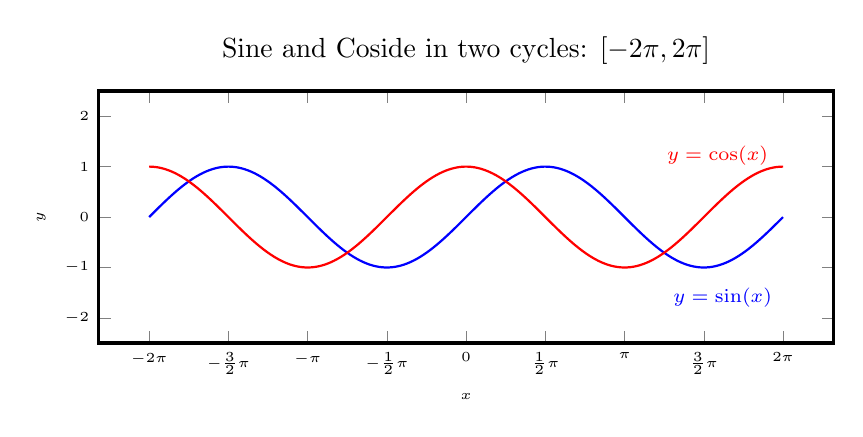
\begin{tikzpicture}
    \begin{axis}[
        width=0.9\textwidth,
        axis line style={very thick,-stealth},
        xmin=-2*pi-0.5,xmax=2*pi+0.5,ymin=-2,ymax=2,
        ytick={-4,-3,...,3,4},
        xtick={-2*pi,-1.5*pi,-pi,-0.5*pi,0,0.5*pi,pi,1.5*pi,2*pi
        },
        xticklabels={$-2\pi$,$-\frac{3}{2}\pi$,$-\pi$,$-\frac{1}{2}\pi$,$0$,$\frac{1}{2}\pi$,$\pi$,$\frac{3}{2}\pi$,$2\pi$
        },
        tick label style={font=\tiny},
        every axis plot post/.append style={thick},
        label style={font=\tiny},
        xlabel=$x$,
        ylabel=$y$,
        enlargelimits={abs=0.5},
        unit vector ratio*=1 1,
        smooth,
        grid=none,
        title={Sine and Coside in two cycles: $[-2\pi, 2\pi]$}
        ]
    \addplot[domain=-2*pi:2*pi,samples=200,blue]{sin(deg(x))} node[pos=0.9, below=5pt, font=\scriptsize]{$y=\sin(x)$};
    \addplot[domain=-2*pi:2*pi,samples=200,red]{cos(deg(x))} node[pos=0.9,above=10pt, font=\scriptsize]{$y=\cos(x)$};
    \end{axis}
  \end{tikzpicture}
\end{center}

\begin{definition}
  A \textbf{sinusoidal function} is a function $f$ that is defined by
  $f(x)=A\sin(Bx-C)+D$ or $f(x)=A\cos(Bx-C)+D$. The horizontal line $y=D$ is called the \textbf{midline}. The \textbf{amplitude} of $f$ is maximal distance that a value of $f$ can be above or below the midline, that is 
  \[\text{amplitude}=\frac{1}{2}|f_{\max}-f_{\min}|.\]
\end{definition}

\begin{howto}[Characterize Sinusoidal Function]
  Given a sinusoidal function $y=A\sin(Bx-C)+D$ or $y=A\cos(Bx-C)+D$, or equivalently, $y=A\sin(B(x-\frac{C}{B}))+D$ or $y=A\cos(B(x-\frac{C}{B}))+D$, 
  \begin{itemize}
    \item the amplitude is $|A|$;
    \item the period is $\dfrac{2\pi}{B}$;
    \item the phase shift is $\dfrac{C}{B}$;
    \item the midline is $y=D$.
  \end{itemize}
\end{howto}

\newpage

\begin{example}
  Determine the midline, amplitude, period, and phase shift of the function $y=3\sin (2x)+1$.
\end{example}

\begin{example}
  Sketch a graph of $f(x)=-2\sin\left(\dfrac{\pi x}{2}\right)$.
\end{example}

\newpage

\begin{example}
  Given $y=-2\cos\left(\dfrac{\pi}{2}x+\pi\right)+3$, determine the amplitude, period, phase shift, and midline. Then graph the function.
\end{example}

\begin{example}
  Find an equation of the sinusoidal function defined by the following graph.\\
  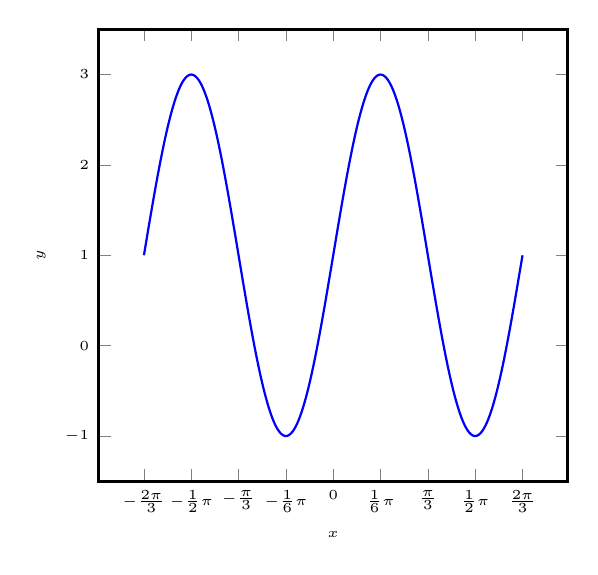
\begin{tikzpicture}
    \begin{axis}[
        width=0.7\textwidth,
        axis line style={very thick,-stealth},
        xmin=-2*pi/3,xmax=2*pi/3,ymin=-1,ymax=3,
        ytick={-4,-3,...,4,5},
        xtick={-2/3*pi,-1.5/3*pi,-pi/3,-0.5*pi/3,0,0.5*pi/3,pi/3,1.5*pi/3,2*pi/3
        },
        xticklabels={$-\frac{2\pi}{3}$,$-\frac{1}{2}\pi$,$-\frac{\pi}{3}$,$-\frac{1}{6}\pi$,$0$,$\frac{1}{6}\pi$,$\frac{\pi}{3}$,$\frac{1}{2}\pi$,$\frac{2\pi}{3}$
        },
        tick label style={font=\tiny},
        every axis plot post/.append style={thick},
        label style={font=\tiny},
        xlabel=$x$,
        ylabel=$y$,
        enlargelimits={abs=0.5},
        unit vector ratio*=1 1,
        smooth,
        % grid=none,
        ]
    \addplot[domain=-2*pi/3:2*pi/3,samples=200,blue]{2*sin(deg(3*x))+1};
    \end{axis}
  \end{tikzpicture}
\end{example}
\vspace*{-0.3\textheight}
\newpage

\section*{Exercises}


\begin{exercise}
  Determine the midline, amplitude, period, and phase shift of the function $y=2\cos(2\pi x-\pi)-1$.
\end{exercise}

\begin{exercise}
  Given $y=-3\sin\left(\dfrac{\pi}{2}x-\pi\right)+2$, determine the amplitude, period, phase shift, and midline. Then graph the function.
\end{exercise}

\begin{exercise}
  Find an equation of the sinusoidal function defined by the following graph.\\
  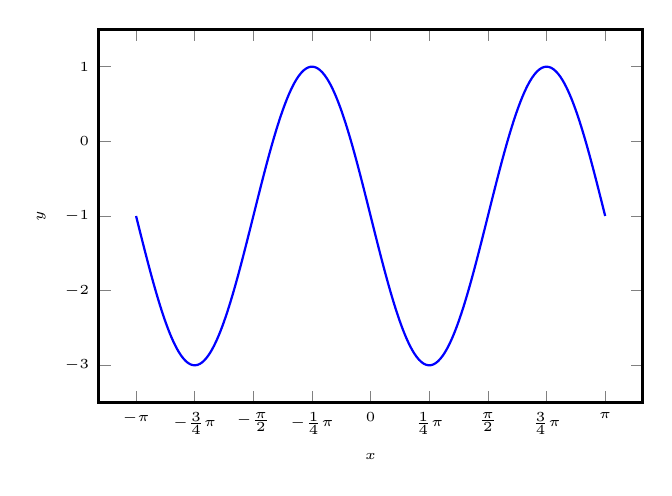
\begin{tikzpicture}
    \begin{axis}[
        width=0.7\textwidth,
        axis line style={very thick,-stealth},
        xmin=-pi,xmax=pi,ymin=-3,ymax=1,
        ytick={-4,-3,...,4,5},
        xtick={-pi,-1.5/2*pi,-pi/2,-0.5*pi/2,0,0.5*pi/2,pi/2,1.5*pi/2,2*pi/2
        },
        xticklabels={$-\pi$,$-\frac{3}{4}\pi$,$-\frac{\pi}{2}$,$-\frac{1}{4}\pi$,$0$,$\frac{1}{4}\pi$,$\frac{\pi}{2}$,$\frac{3}{4}\pi$,$\pi$
        },
        tick label style={font=\tiny},
        every axis plot post/.append style={thick},
        label style={font=\tiny},
        xlabel=$x$,
        ylabel=$y$,
        enlargelimits={abs=0.5},
        unit vector ratio*=1 1,
        smooth,
        % grid=none,
        ]
    \addplot[domain=-pi:pi,samples=200,blue]{-2*sin(deg(2*x))-1};
    \end{axis}
  \end{tikzpicture}
\end{exercise}

\newpage

\section{Graph of Other Trigonometric Functions}

\begin{howto}[Graph of $y = A \tan(Bx)$]
  \begin{itemize}
    \item The stretching factor is $|A|$.
    \item The period is $P=\dfrac{\pi}{|B|}$.
    \item The domain consists of all real numbers $x$ such that $x\ne \dfrac{(2k+1)\pi}{|B|}$ for all integer $k$.
    \item The range is $(-\infty,\infty)$.
    \item The vertical asymptote $x=\dfrac{(2k+1)\pi}{|B|}$.
    \item The function is an odd function.
    \item The $y$-intercept is $(0, 0)$.
    \item The $x$-intercepts are $(k\pi,0)$.
  \end{itemize}
\end{howto}

\begin{example}
  Sketch a graph of one period of the function  $y=\dfrac{1}{2}\tan\left(\dfrac{\pi}{2}x\right)$.
\end{example}

\begin{note}
The graph of the cotangent function can be obtained from the graph of a tangent function by horizontal shift of $-\dfrac{\pi}{2B}$ units.
\end{note}



\newpage

\begin{howto}[Graph of $y = A \sec(Bx)$]
\begin{itemize}
  \item The stretching factor is $|A|$.
  \item The period is $\dfrac{2\pi}{|B|}$.
  \item The domain consists of all real numbers $x$ such that $x\ne \dfrac{(2k+1)\pi}{2|B|}$, where $k$ is an integer.
  \item The range is $(-\infty,- |A| ]\cup [ |A|,\infty)$
  \item The vertical asymptotes are $x=\dfrac{(2k+1)\pi}{2|B|}$, where $k$ is an integer.
  \item The function is an even function.
\end{itemize}
\end{howto}

\begin{example}
  Sketch a graph of $f(x)=2\sec(\pi x)$ in one period.
\end{example}

\begin{note}
  The graph of the cosecant function can be obtained from the graph of a secant function by a horizontal shift of $\dfrac{\pi}{2B}$ units.
\end{note}

\newpage

\begin{example}
  Find an equation of the tangent function defined by the following graph.\\
  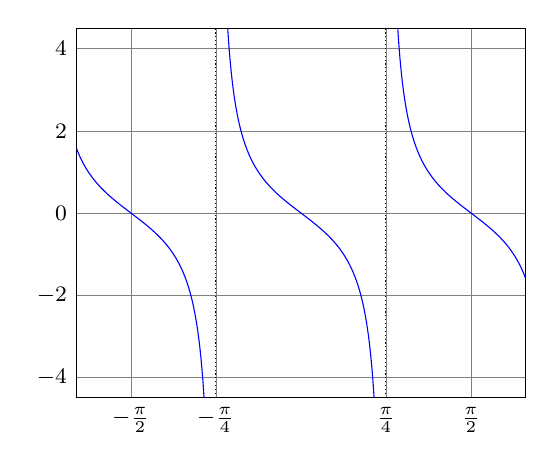
\begin{tikzpicture}
    \begin{axis}[%
      width=0.6\textwidth,
        xmin=-pi/2-0.5,
        xmax=pi/2+0.5,
        ymin=-4.5,
        ymax=4.5,
        grid=both,
        grid style={very thin, gray},
        trig format plots=rad, %<- 
        xtick={-2*pi/2,-3*pi/2/2, -pi/2, -pi/2/2,pi/2/2,pi/2,3*pi/2/2,2*pi/2},
        xticklabels={$-\pi$, $-\frac{3\pi}{4}$, $-\frac{\pi}{2}$, $-\frac{\pi}{4}$, $\frac{\pi}{4}$,$\frac{\pi}{2}$,$\frac{3\pi}{4}$,$\pi$},
        every axis y label/.style={rotate=0, black, at={(0.5,1.05)},},
        every axis x label/.style={rotate=0, black, at={(1.05,0.5)},},,
        font=\footnotesize,     
     ]
    \pgfplotsinvokeforeach{-5,-3,...,3}{
    \pgfmathsetmacro{\xmin}{ifthenelse(#1==-5,-2*pi/2,#1*pi/2/2+0.01)}
    \pgfmathsetmacro{\xmax}{ifthenelse(#1==3,2*pi/2,#1*pi/2/2+pi/2-0.01)}
    \addplot[blue, samples=201,smooth,domain=\xmin:\xmax]{-tan(2*x)};
    \draw[densely dotted] (#1*pi/4,\pgfkeysvalueof{/pgfplots/ymin})
     -- (#1*pi/4,\pgfkeysvalueof{/pgfplots/ymax});
    }
    \end{axis}
    \end{tikzpicture}    
\end{example}

\begin{example}
  Find an equation of the secant function defined by the following graph.\\
  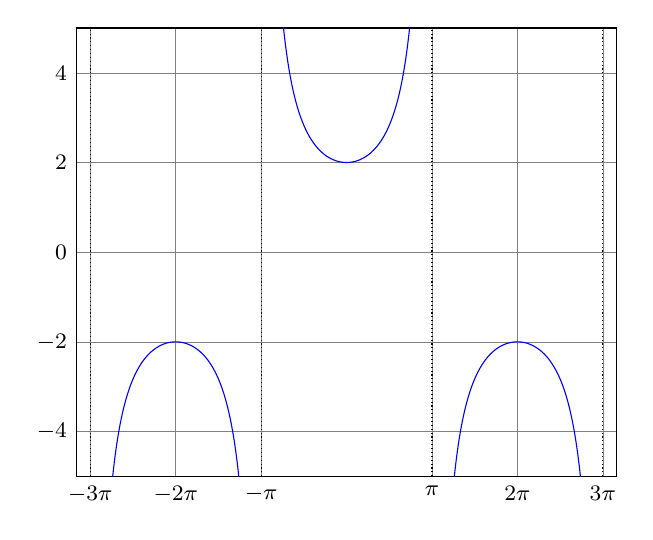
\begin{tikzpicture}
    \begin{axis}[%
        xmin=-3*pi-0.5,
        xmax=3*pi+0.5,
        ymin=-5,
        ymax=5,
        grid=both,
        grid style={very thin, gray},
        trig format plots=rad, %<- 
        xtick={-4*pi,-3*pi, -2*pi, -pi,pi,2*pi,3*pi,4*pi},
        xticklabels={$-4\pi$, $-3\pi$, $-2\pi$, $-\pi$, $\pi$,$2\pi$,$3\pi$,$4\pi$},
        every axis y label/.style={rotate=0, black, at={(0.5,1.05)},},
        every axis x label/.style={rotate=0, black, at={(1.05,0.5)},},,
        font=\footnotesize,     
     ]
    \pgfplotsinvokeforeach{-5,-3,...,3}{
    \pgfmathsetmacro{\xmin}{ifthenelse(#1==-5,-4*pi,#1*pi+0.01)}
    \pgfmathsetmacro{\xmax}{ifthenelse(#1==3,4*pi,#1*pi+2*pi-0.01)}
    \addplot[blue, samples=201,smooth,domain=\xmin:\xmax]{2*sec(x/2)};
    \draw[densely dotted] (#1*pi,\pgfkeysvalueof{/pgfplots/ymin})
     -- (#1*pi,\pgfkeysvalueof{/pgfplots/ymax});
    }
    \end{axis}
    \end{tikzpicture}    
\end{example}

\newpage

\section*{Exercises}

\begin{exercise}
  Sketch a graph of $f(x)=3\tan\left(\dfrac{\pi}{6}x \right)$ in one period.
\end{exercise}

\begin{exercise}
  Sketch a graph of $f(x)=-2\sec\left(4 x \right)$ in one period.
\end{exercise}

\newpage

\begin{exercise}
  Find an equation of the tangent function defined by the following graph.\\
  \begin{tikzpicture}
    \begin{axis}[%
        xmin=-3*pi-0.5,
        xmax=3*pi+0.5,
        ymin=-5,
        ymax=5,
        grid=both,
        grid style={very thin, gray},
        trig format plots=rad, %<- 
        xtick={-3*pi,-2*pi, -pi, pi, 2*pi,3*pi},
        xticklabels={$-3\pi$, $-2\pi$, $-\pi$, $\pi$,$2\pi$,$3\pi$},
        every axis y label/.style={rotate=0, black, at={(0.5,1.05)},},
        every axis x label/.style={rotate=0, black, at={(1.05,0.5)},},,
        font=\footnotesize,     
     ]
    \pgfplotsinvokeforeach{-5,-3,...,3}{
    \pgfmathsetmacro{\xmin}{ifthenelse(#1==-5,-4*pi,#1*pi+0.01)}
    \pgfmathsetmacro{\xmax}{ifthenelse(#1==3,2*pi,#1*pi+2*pi-0.01)}
    \addplot[blue, samples=201,smooth,domain=\xmin:\xmax]{2*tan(x/2)};
    \draw[densely dotted] (#1*pi,\pgfkeysvalueof{/pgfplots/ymin})
     -- (#1*pi,\pgfkeysvalueof{/pgfplots/ymax});
    }
    \end{axis}
    \end{tikzpicture}    
\end{exercise}

\begin{exercise}
  Find an equation of the secant function defined by the following graph.\\
  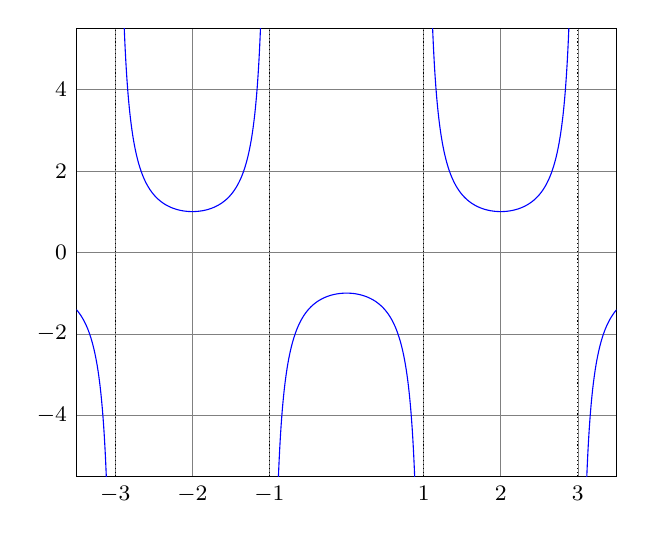
\begin{tikzpicture}
    \begin{axis}[%
        xmin=-3-0.5,
        xmax=3+0.5,
        ymin=-5.5,
        ymax=5.5,
        grid=both,
        grid style={very thin, gray},
        trig format plots=rad, %<- 
        xtick={-4,-3, -2, -1,1,2,3,4},
        xticklabels={$-4$, $-3$, $-2$, $-1$, $1$,$2$,$3$,$4$},
        every axis y label/.style={rotate=0, black, at={(0.5,1.05)},},
        every axis x label/.style={rotate=0, black, at={(1.05,0.5)},},
        font=\footnotesize,     
     ]
    \pgfplotsinvokeforeach{-5,-3,...,3}{
    \pgfmathsetmacro{\xmin}{ifthenelse(#1==-5,-4,#1+0.01)}
    \pgfmathsetmacro{\xmax}{ifthenelse(#1==3,4,#1+2-0.01)}
    \addplot[blue, samples=201,smooth,domain=\xmin:\xmax]{-sec(pi*x/2)};
    \draw[densely dotted] (#1,\pgfkeysvalueof{/pgfplots/ymin})
     -- (#1,\pgfkeysvalueof{/pgfplots/ymax});
    }
    \end{axis}
    \end{tikzpicture}    
\end{exercise}

\newpage
\section{Inverse Trigonometric Functions}

\begin{definition}
  On restricted domains, we can define the inverse trigonometric functions.
  \begin{itemize}
    \item The inverse sine function $y={\sin}^{-1}x$ means $x=\sin y$. The inverse sine function is sometimes called the \textbf{arcsine} function , and notated $\arcsin x$. $y={\sin}^{-1}x$ has domain $[-1,1]$ and range $\left[-\frac{\pi}{2},\frac{\pi}{2}\right]$.
  
    \item The inverse cosine function $y={\cos}^{-1}x$ means $x=\cos y$. The inverse cosine function is sometimes called the \textbf{arccosine} function, and notated $\arccos x$. $y={\cos}^{-1}x$ has domain $[-1,1]$ and range $[0,\pi]$.
  
    \item The inverse tangent function $y={\tan}^{-1}x$ means $x=\tan y$. The inverse tangent function is sometimes called the \textbf{arctangent} function, and notated $\arctan x$. $y={\tan}^{-1}x$ has domain $(-\infty,\infty)$ and range $\left(-\frac{\pi}{2},\frac{\pi}{2}\right)$.
  \end{itemize}
\end{definition}

\begin{example}
Evaluate each of the following.\\
\begin{enumerate*}
    \item ${\sin}^{-1}\left(-\dfrac{\sqrt{2}}{2}\right)$
    \item ${\cos}^{-1}\left(-\dfrac{\sqrt{3}}{2}\right)$
    \item ${\tan}^{-1}(1)$\hfill\null
\end{enumerate*}
\end{example}

\newpage

\begin{example}
  Solve the angle $\theta$ (rounded to the hundredth radian) from the given right triangle.

  \begin{tikzpicture}
    \tkzDefPoints{0/0/A,{5*cos((atan(5/12)))}/0/B,{5*cos((atan(5/12)))}/{5*sin((atan(5/12)))}/C}
    \tkzDrawPolygons(A,B,C)
    \tkzLabelAngle[pos=1](B,A,C){$\theta$}
    \tkzMarkAngle[size=0.6](B,A,C)
    % \tkzLabelSegment[auto](A,C){$12$}
    \tkzLabelSegment[auto,swap](A,B){$12$}
    \tkzLabelSegment[auto,swap](B,C){$5$}
    \tkzMarkRightAngles(C,B,A)
  \end{tikzpicture}
\end{example}


\begin{howto}[The Composition of a Trigonometric Function and an Inverse Trigonometric Function]
From the definition of inverse function, we know
$$
\begin{aligned} 
  \sin({\sin}^{-1}x)&= x\qquad \text{for } -1\leq x\leq 1\\ 
  \cos({\cos}^{-1}x)&= x\qquad \text{for } -1\leq x\leq 1\\ 
  \tan({\tan}^{-1}x)&= x\qquad \text{for } -\infty<x<\infty\\ 
  {\sin}^{-1}(\sin x)&= x\qquad \text{only for } -\dfrac{\pi}{2}\leq x\leq \dfrac{\pi}{2}\\ 
  {\cos}^{-1}(\cos x)&= x\qquad \text{only for } 0\leq x\leq \pi\\ 
  {\tan}^{-1}(\tan x)& =x\qquad \text{only for } -\dfrac{\pi}{2}< x< \dfrac{\pi}{2}.
\end{aligned}
$$
The trigonometric identities may also need to when the functions in the composition are not inverse to each other.
\end{howto}

\begin{example}
  Evaluate the following.\\
  \begin{enumerate*}
    \item ${\sin}^{-1}\left(\sin \left(\dfrac{\pi}{3}\right)\right)$
    \item ${\cos}^{-1}\left(\cos \left(-\dfrac{\pi}{3}\right)\right)$\hfill\null
  \end{enumerate*}
\end{example}

\newpage

\begin{example}
  Evaluate $\sin^{-1}\left(\cos\left(\dfrac{13\pi}{6}\right)\right)$.
\end{example}

\begin{example}
  Find an exact value for $\sin\left({\cos}^{-1}\left(\dfrac{4}{5}\right)\right)$
\end{example}

\begin{example}
  Find an exact value for $\sin\left({\tan}^{-1}\left(\dfrac{7}{4}\right)\right)$.
\end{example}

\newpage
\section*{Exercises}


\begin{exercise}
  Evaluate each of the following.\\
  \begin{enumerate*}
      \item ${\sin}^{-1}\left(\dfrac{\sqrt{3}}{2}\right)$
      \item ${\cos}^{-1}\left(-\dfrac{1}{2}\right)$
      \item ${\tan}^{-1}(-\sqrt{3})$\hfill\null
  \end{enumerate*}
  \end{exercise}
  
  \begin{exercise}
    Solve the angle $\theta$ (rounded to the hundredth radian) from the given right triangle.
  
    \begin{tikzpicture}
      \tkzDefPoints{0/0/A,{5*cos((asin(8/13)))}/0/B,{5*cos((asin(8/13)))}/{5*sin((asin(8/13)))}/C}
      \tkzDrawPolygons(A,B,C)
      \tkzLabelAngle[pos=1](B,A,C){$\theta$}
      \tkzMarkAngle[size=0.6](B,A,C)
      \tkzLabelSegment[auto](A,C){$13$}
      % \tkzLabelSegment[auto,swap](A,B){$8$}
      \tkzLabelSegment[auto,swap](B,C){$8$}
      \tkzMarkRightAngles(C,B,A)
    \end{tikzpicture}
  \end{exercise}
 

  \begin{exercise}
    Evaluate the following.\\
    \begin{enumerate*}
      \item ${\sin}^{-1}\left(\sin \left(\dfrac{\pi}{6}\right)\right)$
      \item ${\cos}^{-1}\left(\cos \left(-\dfrac{\pi}{4}\right)\right)$\hfill\null
    \end{enumerate*}
  \end{exercise}

   
  \newpage
  
  \begin{exercise}
    Evaluate $\cos^{-1}\left(\sin\left(\dfrac{11\pi}{3}\right)\right)$.
  \end{exercise}
  
  \begin{exercise}
    Find an exact value for $\sin\left({\cos}^{-1}\left(\dfrac{3}{5}\right)\right)$
  \end{exercise}
  
  \begin{exercise}
    Find an exact value for $\cos\left({\tan}^{-1}\left(\dfrac{5}{4}\right)\right)$.
  \end{exercise}
  